% homework template
\documentclass[a4paper,11pt]{article}

%package declarations:
%geometry:set the geometry of page
%ragged2e: left/right justify
%fancyhdr: header/footers
\usepackage{geometry}
\usepackage{ragged2e}
\usepackage{fancyhdr}
\usepackage{amsmath,amssymb,amsthm,graphicx}
\usepackage{algorithm}
\usepackage{algpseudocode}
\usepackage{wrapfig}
\usepackage{epsfig}
\usepackage{float}

%redefine maketitle
%http://tex.stackexchange.com/questions/85343/left-align-abstract-title-and-authors
\renewcommand{\maketitle}{%
	
	\Large
 	\textbf{CS 204, Spring 2017}
 	\hfill
 	Multipath-TCP Assignment
 	\par
 	
	\Large
	Abhishek Kumar SRIVASTAVA
	\hfill
	\normalsize
	\today
 	\par
 	Student ID: 861307778
 	\par
 	
 	%plagiarism statement
 	%\begin{center}

 	%\vspace{.2in}
 	
 	%\textit{I certify that this submission represents my own original work }
 	%\par
	%\vspace{.2in}
	%\makebox[2.4in]{\hrulefill}
	%\par

 	%\end{center}
 	
 	\hrulefill
 	\par \vspace{2ex}
 	}


%since using the assignment class, set the geometry
\geometry{total={210mm,297mm},
	left=25mm,right=25mm,%
	bindingoffset=0mm, top=20mm,bottom=20mm}

%set headers and footers
\pagestyle{fancy}
\fancyhf{}
\fancyhead[LE,RO]{\textbf{CS 204:} MPTCP-Assignment}
\fancyhead[RE,LO]{Abhishek Kumar Srivastava}
\fancyfoot[CE,CO]{\leftmark}
\fancyfoot[LE,RO]{\thepage}

%some custom commands, taken from stanford template
\newtheoremstyle{quest}{\topsep}{\topsep}{}{}{\bfseries}{}{ }{\thmname{#1}\thmnote{ #3}.}
\theoremstyle{quest}
\newtheorem*{definition}{Definition}
\newtheorem*{theorem}{Theorem}
\newtheorem*{question}{Question}
\newtheorem*{exercise}{Exercise}
\newtheorem*{challengeproblem}{Challenge Problem}
\newenvironment{solution}[2][Solution]{\begin{trivlist}
		\item[\hskip \labelsep {\bfseries #1}\hskip \labelsep {\bfseries #2.}]}{\end{trivlist}}

\begin{document}\thispagestyle{empty}
	
\maketitle

\begin{solution}
\textbf{Setup Screenshots}:

\begin{figure}[h]
	\centering
	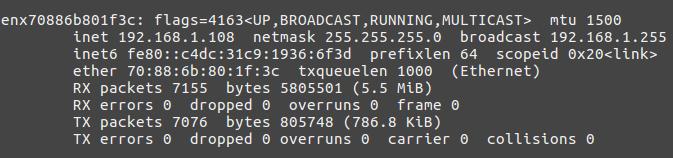
\epsfig{file=N_1_1_1.png, height=2in, width=6in}
	\caption{Ethernet Interface.}
\end{figure}	
\begin{figure}[h]
	\centering
	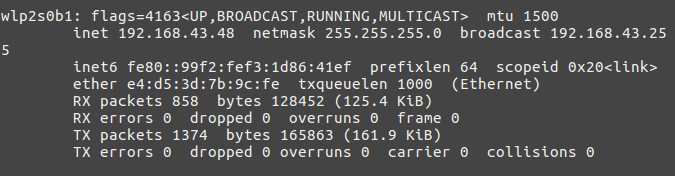
\epsfig{file=N_1_1_2.png, height=2in, width=6in}
	\caption{Wifi Interface 1.}
\end{figure}	

\begin{figure}[h]
	\centering
	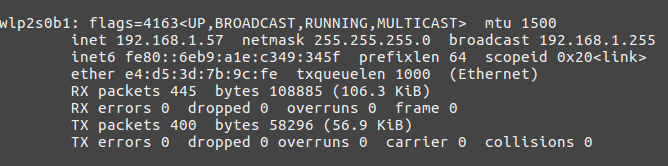
\epsfig{file=N_1_2_1.png, height=2in, width=6in}
	\caption{Wifi Interface 2.}
\end{figure}
\begin{figure}[h]
	\centering
	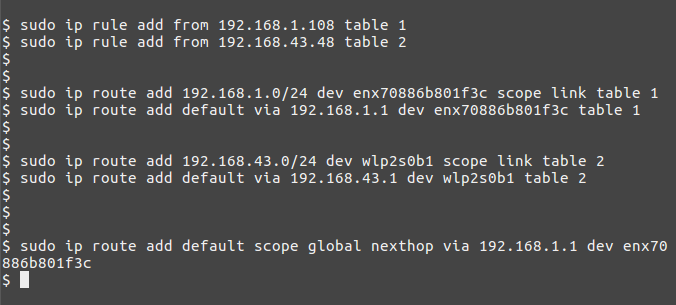
\epsfig{file=N_2.png, height=3in, width=6in}
	\caption{Command to add route table.}
\end{figure}
\begin{figure}[h]
	\centering
	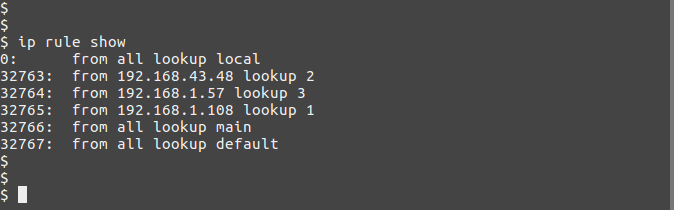
\epsfig{file=N_4_1.png, height=2in, width=6in}
	\caption{IP Rule Show.}
\end{figure}
\begin{figure}[h]
	\centering
	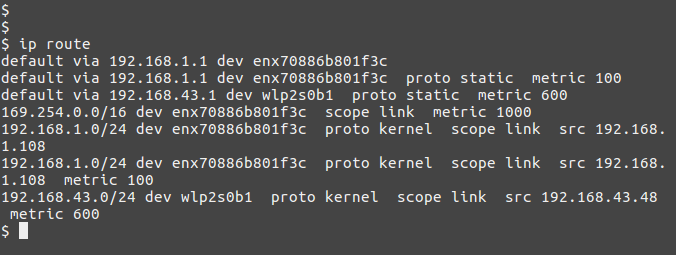
\epsfig{file=N_4.png, height=3in, width=6in}
	\caption{Routing Tables.}
\end{figure}
\begin{figure}[h]
	\centering
	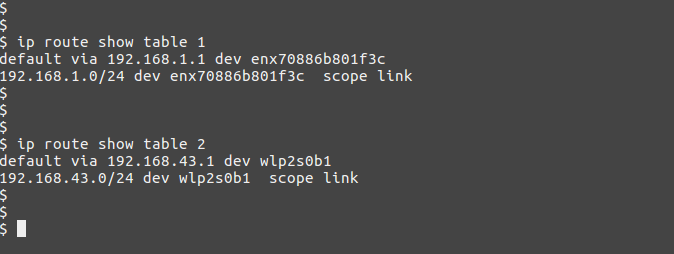
\epsfig{file=N_5.png, height=2.5in, width=6in}
	\caption{IP Route for table 1 \& 2.}
\end{figure}
\begin{figure}[h]
	\centering
	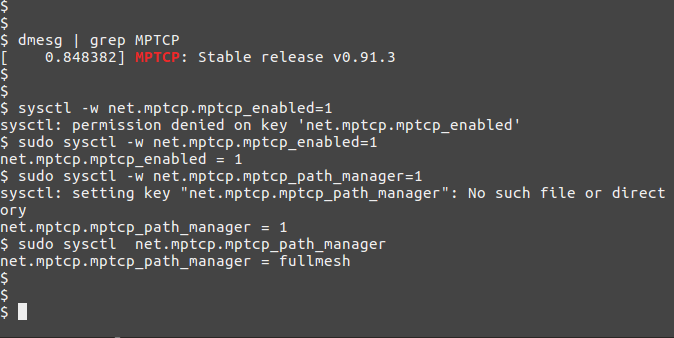
\epsfig{file=N_6.png, height=3.5in, width=6in}
	\caption{Enabling MPTCP and Path Manager.}
\end{figure}
\begin{figure}[h]
	\centering
	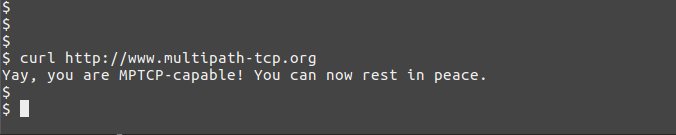
\epsfig{file=N_7.png, height=1.4in, width=6in}
	\caption{MPTCP Enabling Testing.}
\end{figure}
\begin{figure}[h]
	\centering
	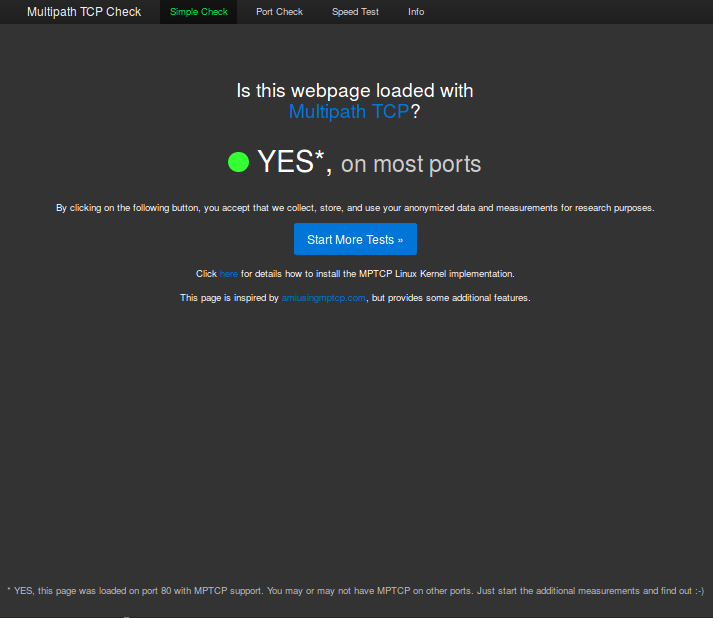
\epsfig{file=N_10.png, height=4.5in, width=6in}
	\caption{MPTCP Enabling Testing.}
\end{figure}
\begin{figure}[h]
	\centering
	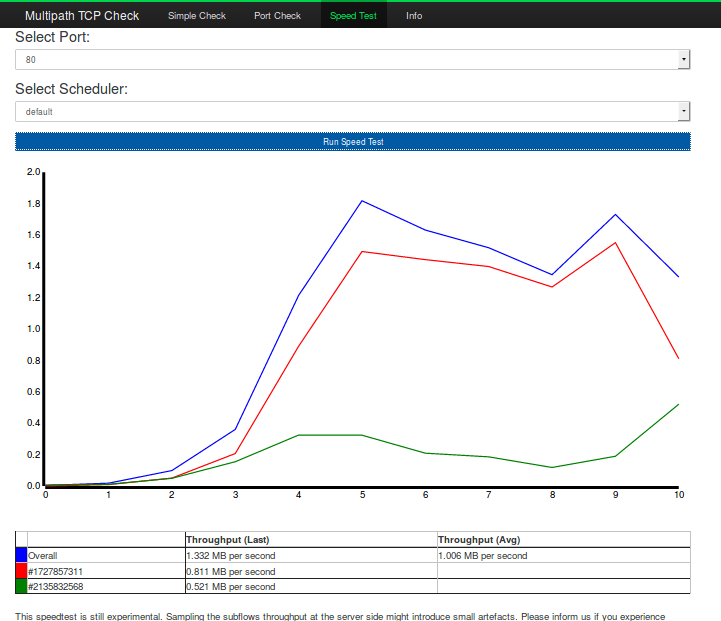
\epsfig{file=N_12_1.png, height=4.5in, width=6in}
	\caption{MPTCP Speed Test:1}
\end{figure}
\begin{figure}[h]
	\centering
	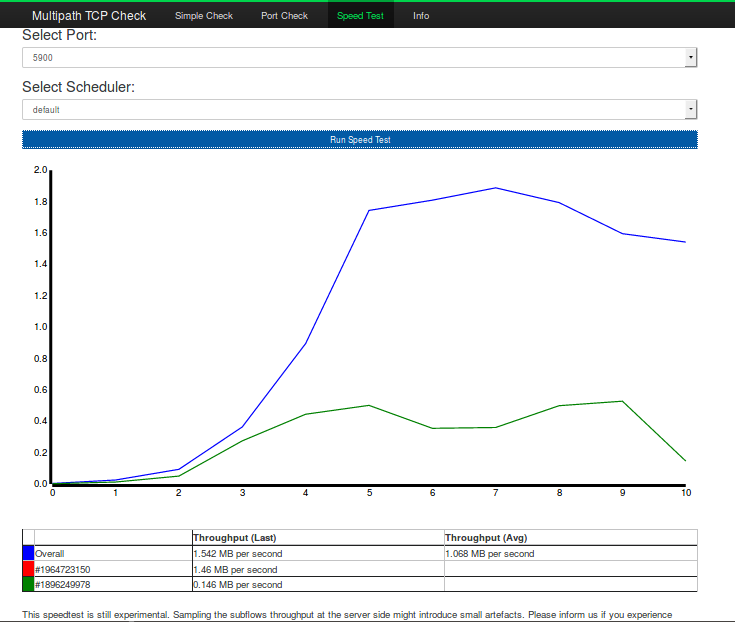
\epsfig{file=N_12_2.png, height=4.5in, width=6in}
	\caption{MPTCP Speed Test:2}
\end{figure}
\begin{figure}[h]
	\centering
	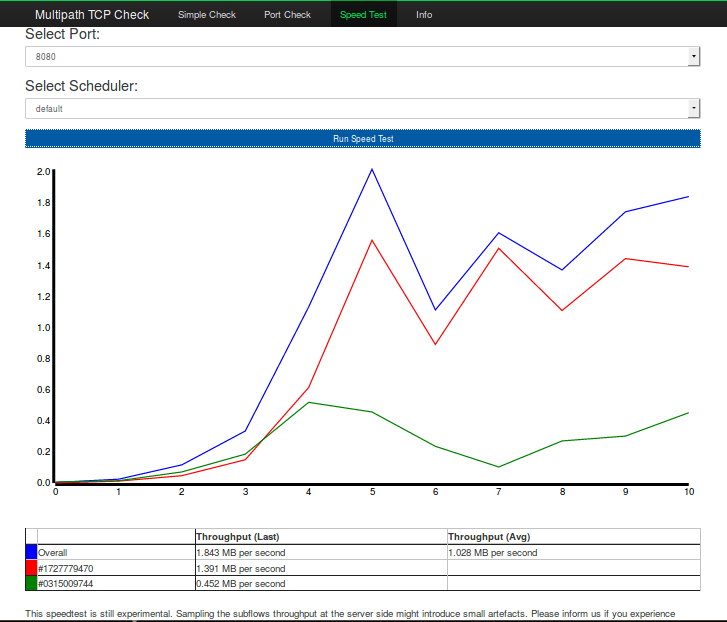
\epsfig{file=N_12_3.png, height=4.5in, width=6in}
	\caption{MPTCP Speed Test:3}
\end{figure}

\end{solution}

\begin{figure}[h]
	\centering
	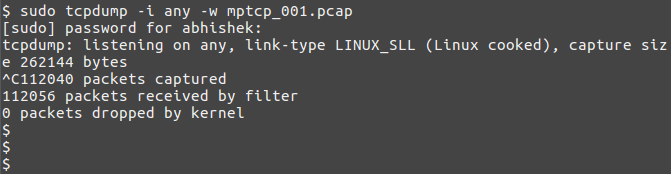
\epsfig{file=N_11.png, height=2in, width=6in}
	\caption{Capturing pcap using tcpdump for mptcp interfaces.}
\end{figure}

\begin{figure}[h]
	\centering
	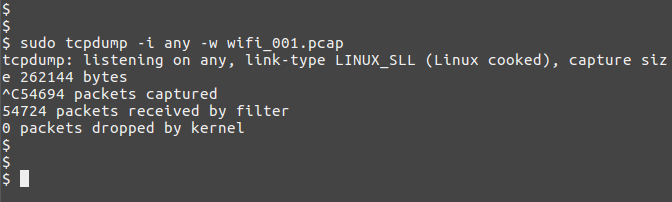
\epsfig{file=N_11_1.png, height=2in, width=6in}
	\caption{Capturing pcap using tcpdump for wifi interface.}
\end{figure}

\begin{figure}[h]
	\centering
	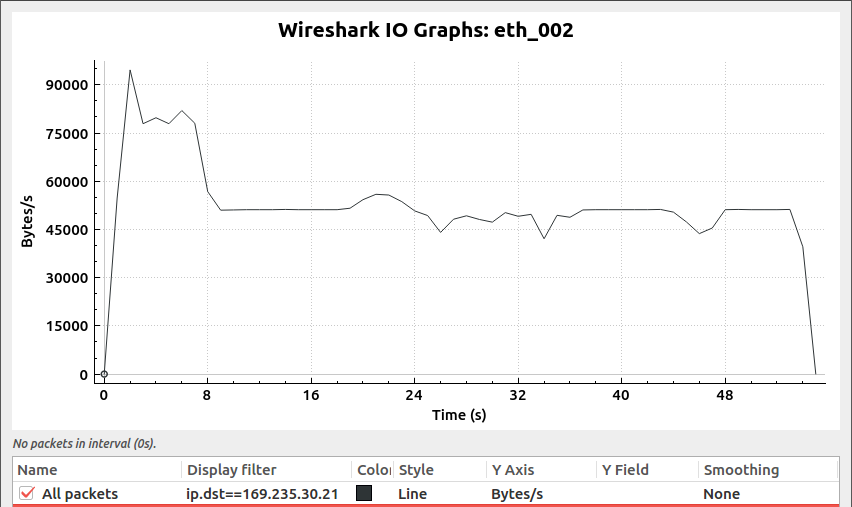
\epsfig{file=N_13_1.png, height=4in, width=6in}
	\caption{Through put using Ethernet interface only.}
\end{figure}

\begin{figure}[h]
	\centering
	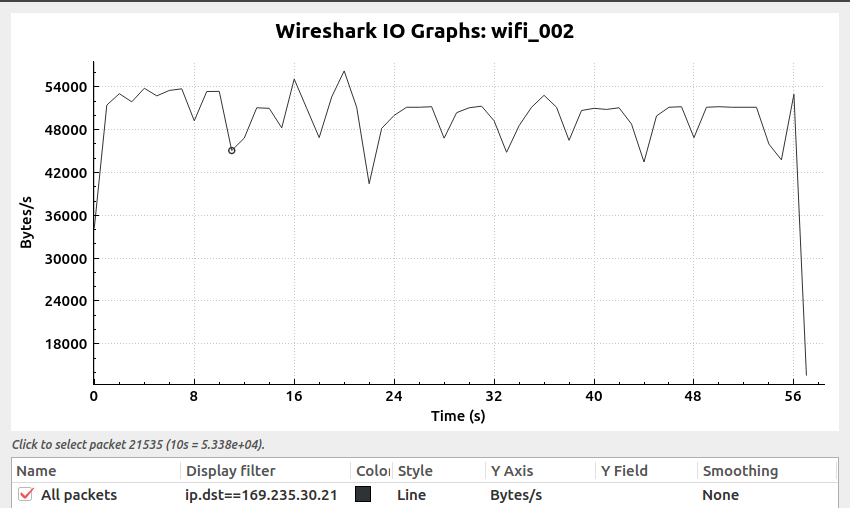
\epsfig{file=N_13_2.png, height=4in, width=6in}
	\caption{Through put using Wifi interface only.}
\end{figure}
\begin{figure}[h]
	\centering
	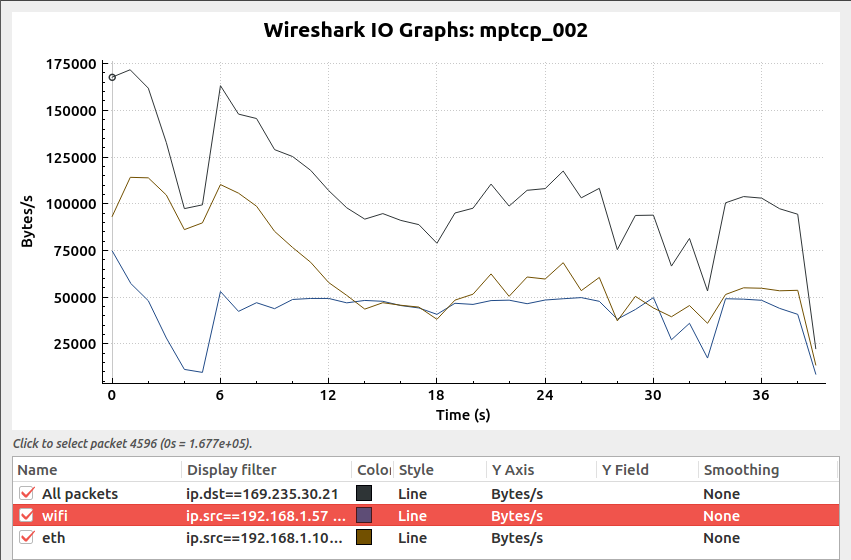
\epsfig{file=N_13_3.png, height=4in, width=6in}
	\caption{Through put using MPTCP interface}
\end{figure}
\begin{figure}[h]
	\centering
	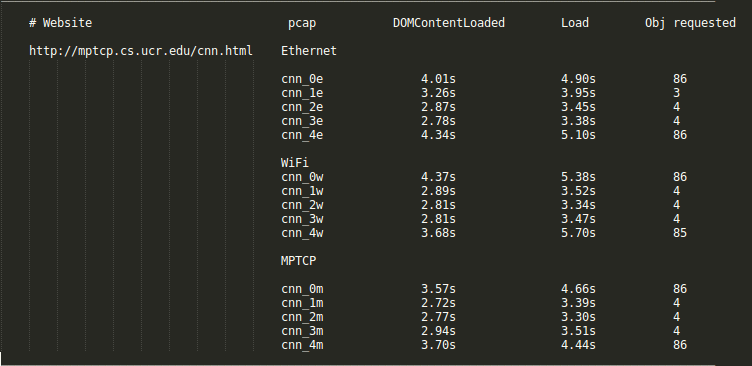
\epsfig{file=N_15_1.png, height=3in, width=6in}
	\caption{Table for CNN Website load for Ethernet, Wifi and MPTCP interface.}
\end{figure}
\begin{figure}[h]
	\centering
	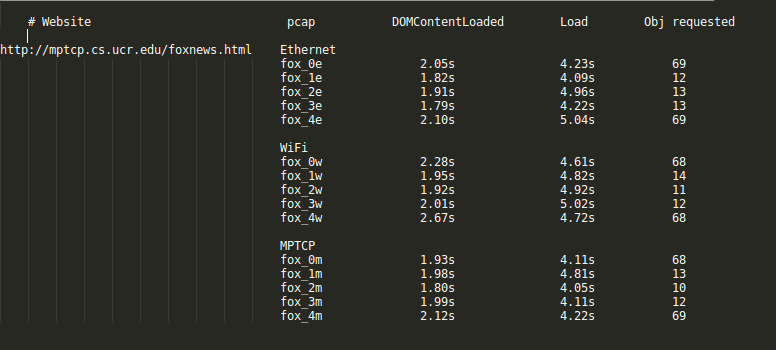
\epsfig{file=N_15_2.png, height=3in, width=6in}
	\caption{Table for Fox Website load for Ethernet, Wifi and MPTCP interface.}
\end{figure}
\begin{figure}[h]
	\centering
	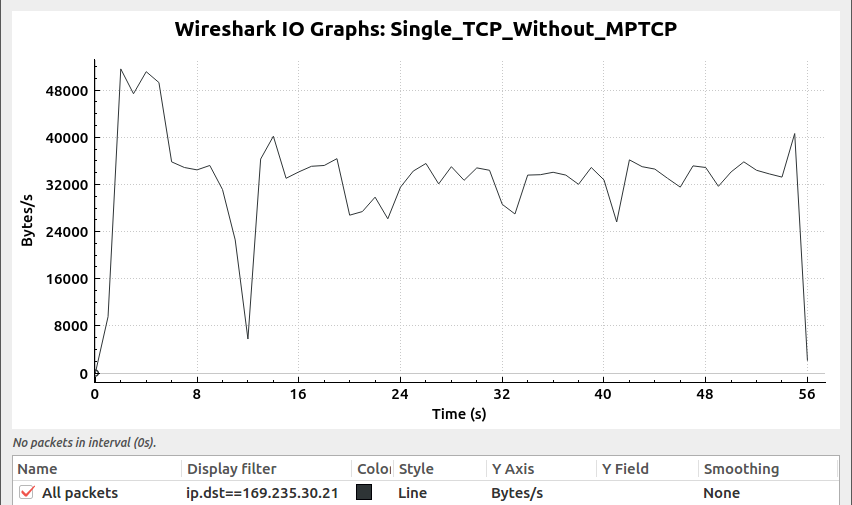
\epsfig{file=N_14_0.png, height=4in, width=6in}
	\caption{Throughput of Single TCP without MPTCP connection.}
\end{figure}
\begin{figure}[h]
	\centering
	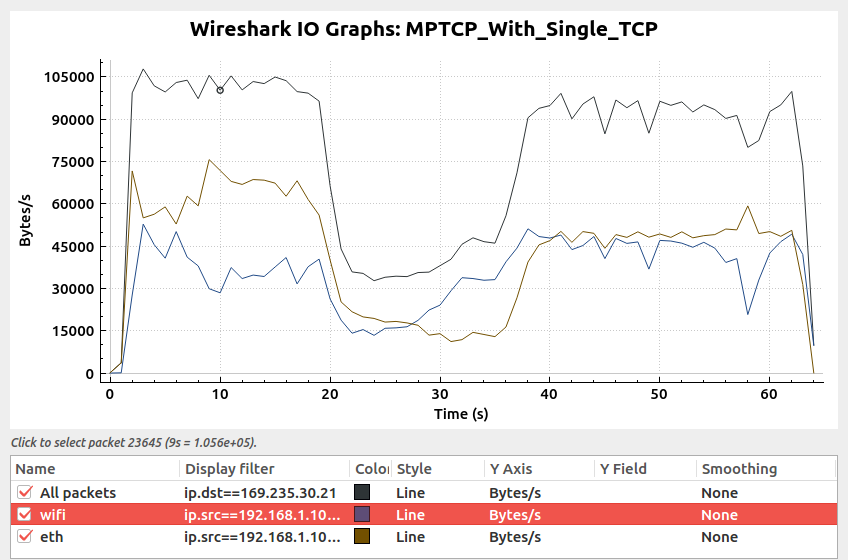
\epsfig{file=N_14_1.png, height=4in, width=6in}
	\caption{Throughput of MPTCP with Single TCP connection.}
\end{figure}
\begin{figure}[h]
	\centering
	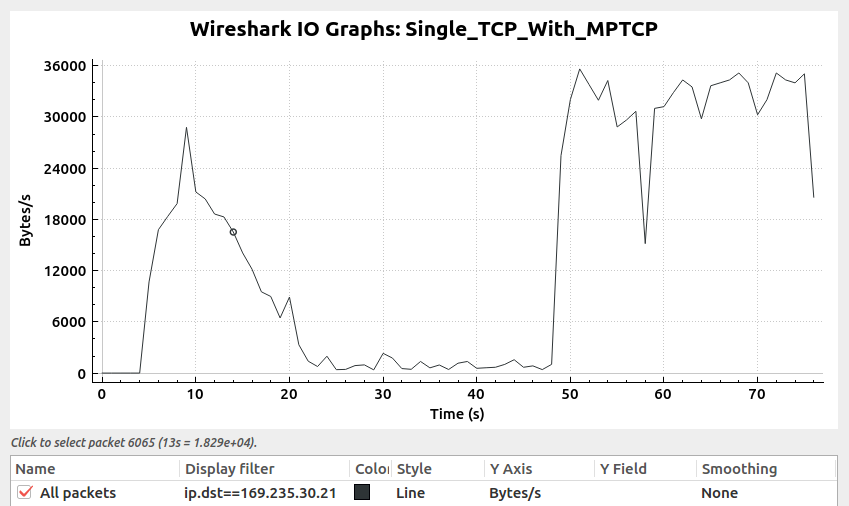
\epsfig{file=N_14_2.png, height=4in, width=6in}
	\caption{Throughput of single TCP in presence of MPTCP connection.}
\end{figure}

\begin{figure}[h]
	\centering
	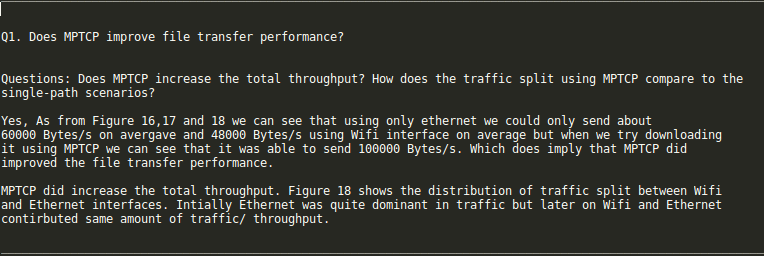
\epsfig{file=N_A_1.png, height=2.7in, width=6in}
	\caption{Answer 1.}
\end{figure}
\begin{figure}[h]
	\centering
	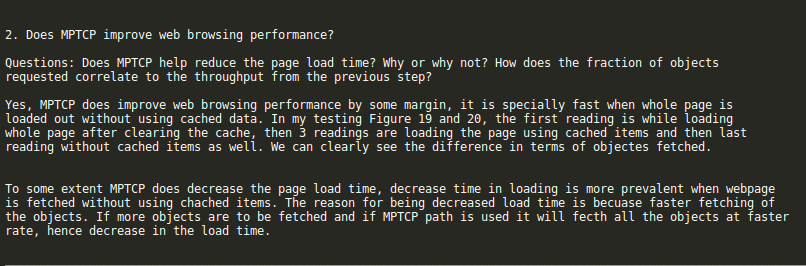
\epsfig{file=N_A_2.png, height=2.8in, width=6in}
	\caption{Answer 2.}
\end{figure}
\begin{figure}[h]
	\centering
	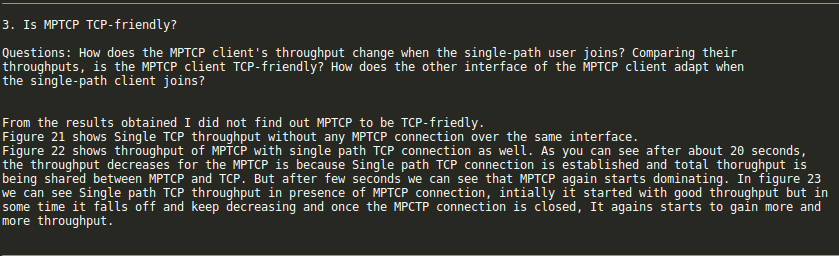
\epsfig{file=N_A_3.png, height=2.7in, width=6in}
	\caption{Answer 3.}
\end{figure}

\end{document}